\documentclass[nonav,sleutel]{beamer}
\usepackage[utf8]{inputenc}
\usepackage[T1]{fontenc}
\title{Politicians and Nobel Prizes}
\date[ISPN '80]{Prof. Dr. Bettina Berendt\\ Knowledge \& the Web 2015-2016}
\author{Katrien Laenen \and Gust Verbruggen \and Ward Schodts}

\usetheme{kuleuvenstijl}

\usepackage{float}
\usepackage{graphicx}
\usepackage{caption}
\usepackage{subcaption}
\graphicspath{ {images/} }

\begin{document}

\begin{frame}
\titlepage
\end{frame}


\begin{frame}[noframenumbering]
\frametitle{Outline} 
  \tableofcontents[hideallsubsections
  ]

\end{frame}

\AtBeginSection[]
{
 \begin{frame}<beamer>
 \frametitle{Outline}
 \tableofcontents[hideothersubsections,currentsection]
 \end{frame}
}


\section{Introduction}
\subsection{Some history}
\begin{frame}
\frametitle{Some history}
\framesubtitle{Nobelprizes, what are they?}
\begin{center}


\begin{figure}[H]    
    \begin{subfigure}[b]{0.33\textwidth}
        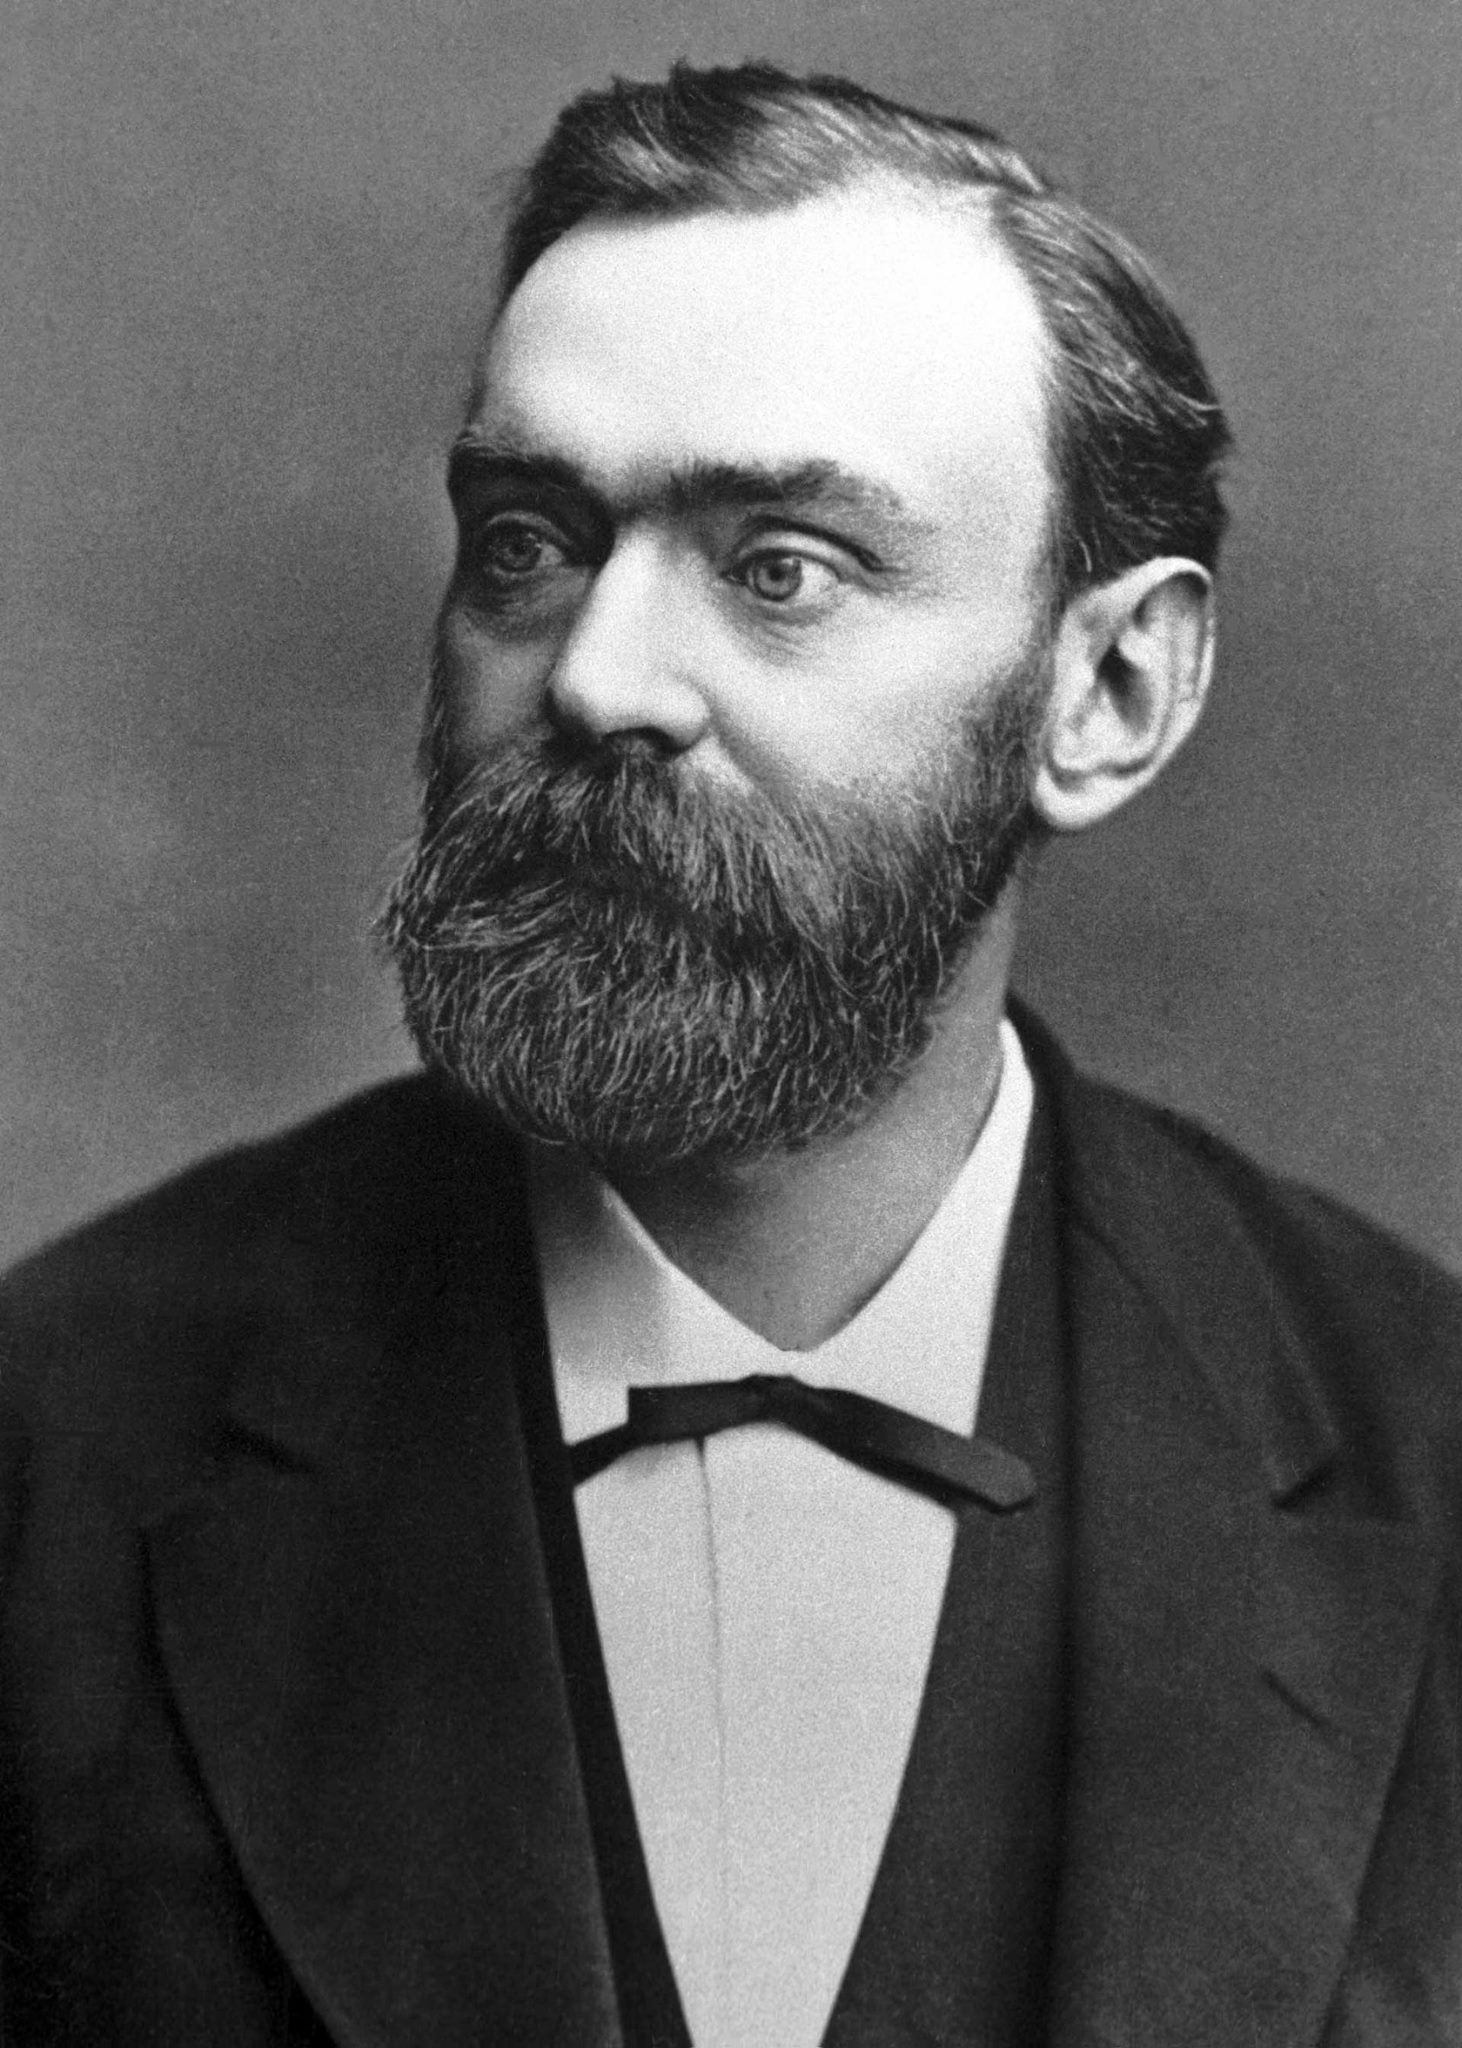
\includegraphics[width=\textwidth]{alfred.jpg}
        \caption{Alfred Nobel}
    \end{subfigure}
    \hspace{2cm}
    \begin{subfigure}[b]{0.33\textwidth}
        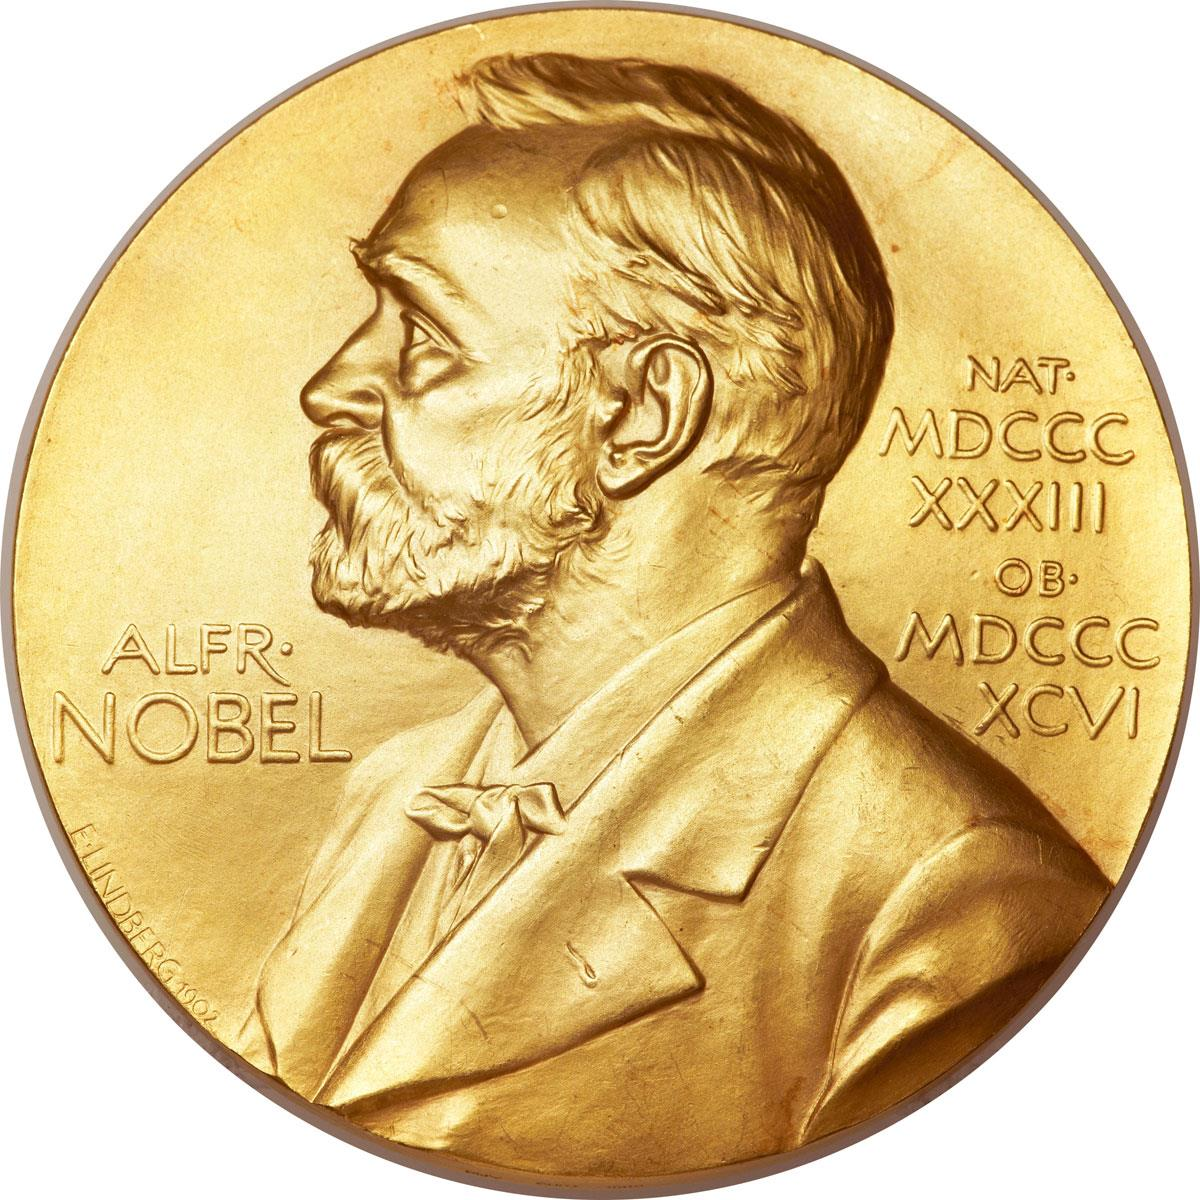
\includegraphics[width=\textwidth]{nobel.jpg}
        \caption{Alfred Nobel}
    \end{subfigure}
\end{figure}
\end{center}
\end{frame}



%%%%%%%%%%%%%%%%%%%%%%%%%%%%%%%%%%%%%%%%%%%%%%%%%%%%%%%%%%%%%%%%%%%%%%%%%%%%%%%%%%%%%%%%%%%%%%%
\subsection{The research question}
\begin{frame}
\frametitle{Our research question} 

\begin{center}
\textit{\Large Which European politicians have a high chance of
receiving a Nobel Prize?}
\end{center}



\end{frame}

\section{Methodology}
\begin{frame}
\frametitle{Methodology}
\framesubtitle{How we will tackle this problem}
\begin{enumerate}
\item<1-> Feature selection: determine features and look for available data
\item<2-> Collecting and combining the data (SPARQL, scraping,...)
\item<3-> Data analysis: learning the model
\item<4-> Interpreting the results
\item<5-> Have a drink
\end{enumerate}
\end{frame}

\section{Data}

\subsection{Feature selection}
\begin{frame}
\frametitle{Feature selection}
\framesubtitle{What features do we look for?}

\begin{enumerate}
\item<1-> Birth year and -place
\item<2-> Award ranking of alma mater
\item<3-> Number of publications $\leftrightarrow$ speeches
\item<4-> Popularity (likes on Facebook)
\item<5-> Nobel Prize: yes/no
\end{enumerate}

\end{frame}

\subsection{Data collection}
\begin{frame}
\frametitle{Data scheme}
\framesubtitle{Where do we get our data?}

\begin{figure}
	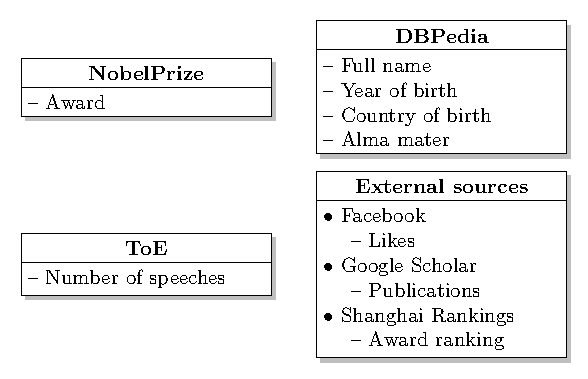
\includegraphics{images/dataschema_original}
\end{figure}

\end{frame}

\begin{frame}
\frametitle{Data scheme}
\framesubtitle{Where do we get our \textbf{training} data?}

\begin{figure}
	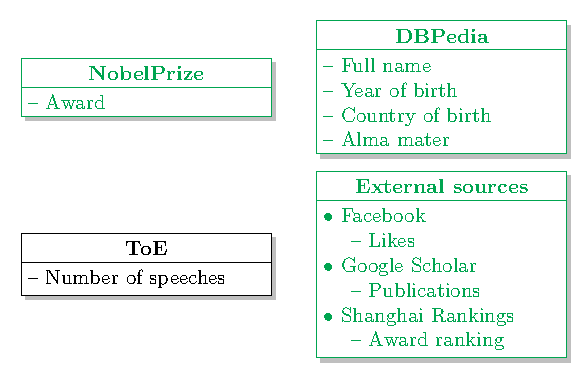
\includegraphics{images/dataschema_training}
\end{figure}

\end{frame}

\begin{frame}
\frametitle{Data scheme}
\framesubtitle{Where do we get our \textbf{research} data?}

\begin{figure}
	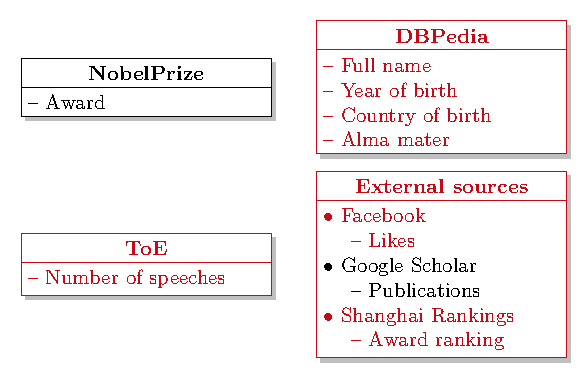
\includegraphics{images/dataschema_research}
\end{figure}

\end{frame}


\section{Analysis}

\subsection{Outlier detection}
\subsection{Learning the model}

\section{Results}

\section{Conclusion}
\begin{frame}
\begin{center}
\Large{Thanks for listening}\\
Any questions?
\end{center}

\end{frame}

\begin{frame}
\frametitle{Our questions}
\begin{enumerate}
\item 
\end{enumerate}
\end{frame}

\end{document}